\documentclass[12pt,xcolor={usenames,dvipsnames}]{beamer}
\usetheme{Hannover}
\setbeamertemplate{footline}[frame number]
\usecolortheme{crane}
\useinnertheme{rectangles}

\usepackage[utf8]{inputenc}
\usepackage[T1]{fontenc}
\usepackage[brazil]{babel}
\usepackage{tipa}
\usepackage{amssymb}
\usepackage{array}
\usepackage{bbold}
\usepackage{latexsym}
\usepackage{ae}
\usepackage{hyperref}
\usepackage{array}
\usepackage{booktabs}
\usepackage{graphicx}
\usepackage{dsfont}
\usepackage{textcomp}
\usepackage{cmll}
\usepackage[normalem]{ulem}
\usepackage{amsmath}
\usepackage{listings}
\usepackage{float}
\usepackage{upgreek}
\usepackage[portuguese]{algorithm2e}
\usepackage{tikz}
\usepackage{multirow}
\usepackage{multicol}
\usetikzlibrary{shapes,arrows,automata,positioning}
\usepackage{stmaryrd}
\newcommand{\CL}{$\mathcal{CL}$\xspace}
%\newcommand{\CLR}{$\mathcal{CL}$ Relativizada\xspace}
\newcommand{\RCL}{$\mathcal{RCL}$\xspace}
\newcommand{\RECALL}{$\mathcal{RECALL}$\xspace}
\newcommand\numberthis{\addtocounter{equation}{1}\tag{\theequation}}

\makeatletter
\newcommand{\miniscule}{\@setfontsize\miniscule{5}{6}}% \tiny: 5/6
\makeatother

\tikzstyle{tech} = [rectangle, draw, text width=7em, text centered]
\tikzstyle{obj} = [rectangle, draw, text width=5em, text centered, rounded corners,  fill=blue!60]  
\tikzstyle{final-logic} = [ellipse, draw, text width=9em, text centered, rounded corners, fill=blue!60]    
\tikzstyle{final-obj} = [rectangle, draw, text width=9em, text centered, rounded corners, fill=blue!60]    
\tikzstyle{line} = [draw, -latex]
\tikzstyle{logic} = [draw, ellipse, text centered]

\setcounter{secnumdepth}{3}
\setcounter{tocdepth}{3}

\lstset{
	backgroundcolor=\color{white},   % choose the background color; you must add \usepackage{color} or \usepackage{xcolor}
	basicstyle=\scriptsize,          % the size of the fonts that are used for the code
	breakatwhitespace=false,         % sets if automatic breaks should only happen at whitespace
	breaklines=true,                 % sets automatic line breaking
	captionpos=b,                    % sets the caption-position to bottom
	columns=flexible,
    deletekeywords={...},            % if you want to delete keywords from the given language
	escapeinside={\%*}{*)},          % if you want to add LaTeX within your code
	extendedchars=true,              % lets you use non-ASCII characters; for 8-bits encodings only, does not work with UTF-8
	frame=none,	                     % adds a frame around the code
	keepspaces=true,                 % keeps spaces in text, useful for keeping indentation of code
	language=Java,                   % the language of the code
	otherkeywords={*,...},           % if you want to add more keywords to the set
	numbers=left,                    % where to put the line-numbers; possible values are (none, left, right)
	numbersep=15pt,                  % how far the line-numbers are from the code
	numberstyle=\tiny,               % the style that is used for the line-numbers
	rulecolor=\color{black},         % if not set, the frame-color may be changed on line-breaks within not-black text
	showspaces=false,                % show spaces everywhere adding particular underscores; it overrides 'showstringspaces'
	showstringspaces=false,          % underline spaces within strings only
	showtabs=false,                  % show tabs within strings adding particular underscores
	stepnumber=1,                    % the step between two line-numbers. If it's 1, each line will be numbered
	tabsize=1	                     % sets default tabsize to 2 spaces
}

\lstdefinelanguage{rcl}{
    keywords=[1]{ O, P, F,CONFLICT,Trace,Stacktrace, AND, \^},
}

\lstdefinestyle{rcl}{
    basicstyle=\normalsize,
    numbers=left,
    numberstyle=\normalsize,
    numbersep=5pt,
    frame=lines,
    breaklines=true,
    prebreak=\raisebox{0ex}[0ex][0ex]{\ensuremath{\hookleftarrow}},
    showstringspaces=false,
    upquote=true,
    tabsize=1,
}

% IMPORTANTE>>> Qualificação: Quarta(16/09/2015) às 15h na sala 311.
% IMPORTANTE>>> Defesa: Quarta(21/09/2016) às 10h na sala 318.

\title[\miniscule{Monitoramento Reativo de Protocolos em Sistemas IoT Sobre o MQTT}]{\textbf{MONITORAMENTO REATIVO DE PROTOCOLOS EM SISTEMAS IOT SOBRE O MQTT}}
\subtitle{}
\author[Gustavo Oliveira Dias] {\textbf{Gustavo Oliveira Dias}}
\institute[CCT-UENP]{Universidade Estadual do Norte do Paraná\\Bacharelado em Ciência da Computação\\\textbf{Orientador: Prof. Me. Wellington Aparecido Della Mura}}
\date[24 de novembro de 2017]{Banca de Defesa do Trabalho de Conclusão de Curso \\ 24 de novembro de 2017}
\subject{Banca de Defesa do Trabalho de Conclusão de Curso - Monitoramento reativo de protocolos em sistemas IoT sobre o MQTT}

\begin{document}
\frame{\titlepage}
\begin{frame}{Roteiro da Apresentação}
    \begin{enumerate}
        \item Motivação;
        \item Formulação e escopo do problema;
        \item Objetivos;
        \item Método proposto;
        \item Estudo de Caso;
        \item Conclusão;
    \end{enumerate}
\end{frame}

\section{Motivação do Trabalho}
\subsection{IoT}
\begin{frame}{Motivação - IoT}
\begin{beamerboxesrounded}{O que é Internet das Coisas?}
	Aplicações que \textbf{armazenam} e \textbf{processam} dados que \\ \textbf{representam virtualmente} objetos do mundo físico, \\ provendo \textbf{interação} e \textbf{comunicação} entre dispositivos \textbf{heterogêneos} conectados.
\end{beamerboxesrounded}
\begin{itemize}
	\item Em 2011, movimentou cerca de US\$44 bi;
	\item Crescimento previsto em US\$290 bi para 2017;
	\item Até 2020, haverá em torno de 34 bi de dispositivos.
	%\item \textbf{Desafio:} lidar com a \textbf{comunicação} entre tantos dispositivos.
	% sensores, dispositivos de rede sem fio, serviços de armazenamento em nuvem, entre outros serviços e dispositivos que compõem este ambiente tecnológico
\end{itemize}
\begin{beamerboxesrounded}{}
\textbf{Desafio:} lidar com a \textbf{comunicação} entre tantos \\ dispositivos conectados.
\end{beamerboxesrounded}
\end{frame}

\subsection{Protocolos}
\begin{frame}{Motivação - Protocolos}
\begin{beamerboxesrounded}{Protocolos de comunicação}
	Conjunto de \textbf{regras-padrão} para \textbf{transmissão de \\ informação} entre computadores.
	\begin{itemize}
		\item Formato;
		\item Sincronização;
		\item Sequência;
		\item Detecção de erros e falhas.
	\end{itemize}
\end{beamerboxesrounded}
\end{frame}

\subsection{MQTT}
\begin{frame}{Motivação - MQTT}
\begin{beamerboxesrounded}{MQTT (\textit{Message Queue Telemetry Transport protocol})}
	Ideal para dispositivos com \textbf{baixo poder de \\ processamento} em ambientes com \textbf{largura de \\ banda limitada}.
\end{beamerboxesrounded}
\textbf{Características}:
\begin{itemize}
	\item Utiliza TCP;
	\item Cabeçalho de apenas 2 bytes;
	\item Estratégia \textit{publish/subscribe};
	\item Clientes se inscrevem em tópicos;
	\item Implementa um servidor próprio: \textit{broker}.
		\item 3 níveis de \textit{Quality of Service} (QoS);
\end{itemize}
\end{frame}

\begin{frame}{Motivação - Protocolos IoT}
\begin{figure}[ht]
	\centering
	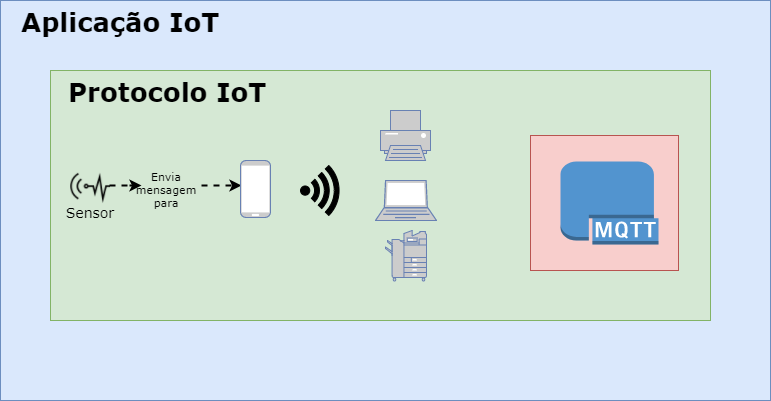
\includegraphics[width=10cm]{./figuras/protocolo_diagrama.png}
\end{figure}    
\end{frame}

\section{Formulação e escopo do problema}
\begin{frame}{Motivação}
\begin{alertblock}{}
É possível \textbf{detectar} e \textbf{identificar} o responsável por uma \textbf{violação} do protocolo?
\end{alertblock}
\quad
\begin{alertblock}{}
	Os protocolos IoT podem ser \textbf{modelados} por meio de \textbf{formalismos}?
\end{alertblock}

\end{frame}

\subsection{Estrutura}
\begin{frame}{Estrutura}
\begin{figure}[ht]
	\centering
	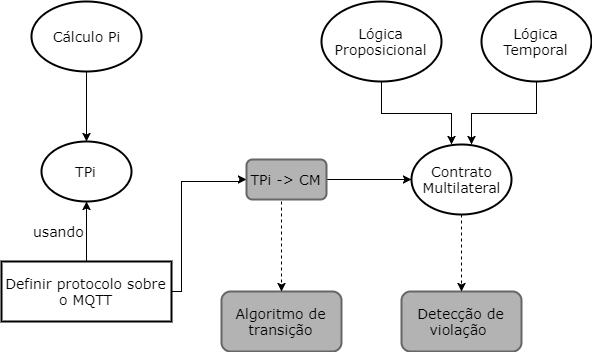
\includegraphics[width=9cm]{./figuras/tcc_estrutura.png}
\end{figure}  
\end{frame}

\section{Objetivos}
\begin{frame}{Objetivos}

\begin{beamerboxesrounded}{Objetivo geral}
Mecanismo para \textbf{formalização} e \textbf{monitoramento \\
	reativo} de sistemas de IoT que utilizam o \\protocolo \textbf{MQTT}.
\end{beamerboxesrounded}
Objetivos específicos:
\begin{itemize}
	\item Definir \textbf{métodos} para representação de protocolos em \textbf{contratos multilaterais} a partir do \textbf{modelo} descrito em \textbf{TPi};
	\item Representar o modelo em TPi do MQTT como um \textbf{contrato multilateral};
	\item Aplicar o algoritmo de monitoramento a um estudo de caso real.
\end{itemize}
\end{frame}

\section{Método Proposto}
\subsection{TPi}
\begin{frame}{Representação formal - TPi}
\begin{beamerboxesrounded}{O que é o TPi?}
	Uma linguagem temporal para modelagem de processos.
\end{beamerboxesrounded}
\begin{align}
&\textbf{QoS~nível~0}~"(At~most~once)":~ \nonumber \\
&\quad Cliente(Publish)~|~Servidor()~|~ClienteSub(),~em~que: \nonumber \\
&\quad Cliente(z) \stackrel{def}{=} \overline{c}\langle z \rangle \nonumber \\
&\quad Servidor() \stackrel{def}{=} c(x).\overline{pub}\langle x \rangle \nonumber \\
&\quad ClienteSub() \stackrel{def}{=} pub(y) \nonumber
\end{align}      
\end{frame}

\subsection{Contratos multilaterais}
\begin{frame}{Contratos multilaterais}
\begin{beamerboxesrounded}{}
	Acordo entre duas ou mais partes baseado em\\ \textbf{compromissos mútuos}.
\end{beamerboxesrounded}
Composto por:
\begin{itemize}
	\item \textbf{Ação:} o que cada parte deverá fazer;
	$$(A\_QoS0enviarPublish, C, S, ?)$$
	\item \textbf{Compromisso:} garantia de cumprimento das ações entre as partes envolvidas;
\end{itemize}	
	\begin{align}
	& c = (C\_QoS0delivery,C,CS,4, \nonumber \\
	& \{ (A\_QoS0enviarPublish,tr), (A\_QoS0receberPublish,fi), \nonumber \\
	& (A\_QoS0publicarPacote,tr), (A\_QoS0receberPacote,fi) \nonumber
	\end{align}
\begin{itemize}	
	\item \textbf{Grafo de compromisso:} forma de visualizar os compromissos entre as partes.
\end{itemize}
\end{frame}

\begin{frame}{QoS 0 - "\textit{At most once}"}

\begin{beamerboxesrounded}{}
	A comunicação baseia-se em um \textit{broker} \textbf{recebendo} e \\\textbf{publicando} mensagens.
\end{beamerboxesrounded}

\begin{table}[!ht]
	\centering\tiny{
		\begin{tabular}{|l|l|l|l|}
			\hline
			\multicolumn{1}{|c|}{\multirow{2}{*}{\textbf{Compromissos}}} & \multicolumn{2}{c|}{\textbf{Classificação das ações e compromissos}} & \multicolumn{1}{c|}{\multirow{2}{*}{\textbf{Rótulos}}} \\ \cline{2-3}
			\multicolumn{1}{|c|}{}                                       & \multicolumn{1}{c|}{$tr$}    & \multicolumn{1}{c|}{$fi$}    & \multicolumn{1}{c|}{}                                  \\ \hline
			$C\_QoS0delivery$                                            & $A\_QoS0enviarPublish$       &                              & $Q0,1$                                                 \\ \cline{2-4} 
			\multicolumn{1}{|c|}{$(Q0)$}                                 &                              & $A\_QoS0receberPublish$      & $Q0,2$                                                 \\ \cline{2-4} 
			& $A\_QoS0publicarPacote$      &                              & $Q0,3$                                                 \\ \cline{2-4} 
			&                              & $A\_QoS0receberPacote$       & $Q0,4$                                                 \\ \hline
		\end{tabular}
	}
\end{table}

\begin{figure}[ht]
	\centering
	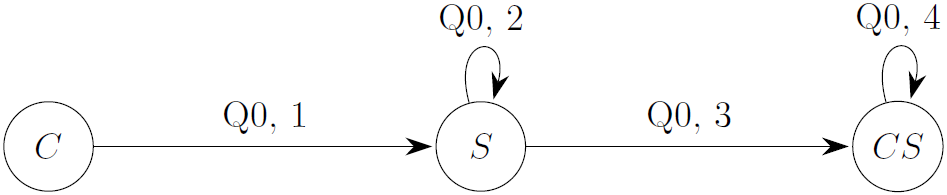
\includegraphics[width=9cm]{./figuras/qos0_grafo.png}
\end{figure} 

\end{frame}

\section{Estudo de caso}
\begin{frame}{Estudo de caso}
\begin{beamerboxesrounded}{}
	Sistema IoT de \textbf{detecção} e \textbf{supressão} de incêndio.
\end{beamerboxesrounded}

\begin{figure}[ht]
	\centering
	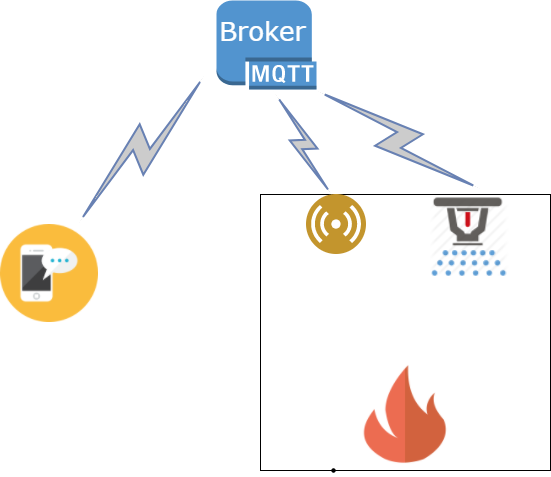
\includegraphics[width=7cm]{./figuras/diagrama_estudo.png}
\end{figure} 
\end{frame}

\begin{frame}{Estudo de caso}
\begin{table}[!ht]
	\centering\tiny{
		\begin{tabular}{|c|c|c|c|c|}
			\hline
			%\rowcolor[HTML]{FFFFFF} 
			{\color[HTML]{000000} \textbf{Mensagem}}                             & {\color[HTML]{000000} \textbf{Tópico MQTT}} & {\color[HTML]{000000} \textit{\textbf{Publisher}}} & {\color[HTML]{000000} \textit{\textbf{Subscriber}}} & {\color[HTML]{000000} \textbf{Ação do \textit{subscriber}}} \\ \hline
			\textit{\begin{tabular}[c]{@{}c@{}}Fire\\ Detection\end{tabular}}    & \textit{Fire/Detected}                      & Sensor de incêndio                                 & \textit{App}                                        & Exibir notificação                                 \\ \hline
			\textit{\begin{tabular}[c]{@{}c@{}}Sprinkler\\ Request\end{tabular}} & \textit{Sprinkler/StReq}                    & \textit{App}                                       & \textit{Sprinkler}                                  & Ler status                                         \\ \hline
			\textit{\begin{tabular}[c]{@{}c@{}}Sprinkler\\ Reply\end{tabular}}   & \textit{Sprinkler/StRep}                    & \textit{Sprinkler}                                 & \textit{App}                                        & Enviar mensagem                                    \\ \hline
			\textit{\begin{tabular}[c]{@{}c@{}}Sprinkler\\ Start\end{tabular}}   & \textit{Sprinkler/Start}                    & \textit{App}                                       & \textit{Sprinkler}                                  & Ativar \textit{sprinkler}                                   \\ \hline
			\textit{\begin{tabular}[c]{@{}c@{}}Sprinkler\\ Start\end{tabular}}   & \textit{Sprinkler/Start}                    & Sensor de incêndio                                 & \textit{Sprinkler}                                  & Ativar \textit{sprinkler}                                   \\ \hline
		\end{tabular}
	}
\end{table}
\end{frame}

\begin{frame}{Estudo de caso}
	\begin{beamerboxesrounded}{O sistema é baseado em três processos, que são \\ \textbf{modelados} e convertidos em um \textbf{contrato}.}
		\begin{itemize}
			\item Detecção/Alerta;
			\item Checagem;
			\item Supressão;
		\end{itemize}
	\end{beamerboxesrounded}
	\begin{itemize}
		\item O \textbf{aplicativo} assume o papél $\textbf{Ap}$ durante a detecção/alerta e checagem, e recebe o papel $\textbf{Ap'}$ no compromisso de supressão;
		\item Os agentes \textbf{broker}, \textbf{sprinkler} e \textbf{sensor} assumem os papéis $\textbf{Br}$, $\textbf{Sp}$ e $\textbf{S}$, respectivamente.
	\end{itemize}
\end{frame}

\subsection{Modelagem e conversão}
\begin{frame}{Estudo de caso - Modelo para Detecção/Alerta}
\begin{align}
& Sensor(FireDetection)~|~Broker()~|~App()~|~Sprinkler(): \nonumber \\
& Sensor(z) \stackrel{def}{=} \overline{fd}\langle z \rangle \nonumber \\
& Broker() \stackrel{def}{=} fd(x).\overline{fd'}\langle x \rangle \nonumber \\
& App() \stackrel{def}{=} fd'(y) \nonumber \\
& Sprinkler() \stackrel{def}{=} fd'(y') \nonumber
\end{align}
\end{frame}

\begin{frame}{Estudo de caso - Conversão do modelo de Detecção/Alerta}

\begin{eqnarray}
Conjunto~de~\textbf{ações}:~\{ &(\overline{fd}\langle z \rangle, S, Br, ?),& \nonumber \\
&(fd(x), Br, Br, ?),& \nonumber \\
&(\overline{fd'}\langle x \rangle, Br, Ap, ?),& \nonumber \\
&(fd'(y), Ap, Ap, ?),& \nonumber \\
&(\overline{fd'2}\langle x \rangle, Br, Sp, ?),& \nonumber \\
&(fd'2(y'), Sp, Sp, ?) \}& \nonumber 
\end{eqnarray}

Compromisso:
\begin{align}
& m_{1} = (C\_detectarIncendio, Sensor, Sprinkler, 6, \nonumber \\
& \{ (\overline{fd}\langle z \rangle, tr), (fd(x), fi), (\overline{fd'}\langle x \rangle, tr), (fd'(y), fi), \nonumber \\ &(\overline{fd'2}\langle x \rangle, tr), (fd'2(y'), fi)~\}) \nonumber
\end{align}

\end{frame}

\begin{frame}{Estudo de caso - Conversão do modelo de Detecção/Alerta}
	\begin{enumerate}
		\item Atribuir um nome ao compromisso;
		$$name = C\_detectarIncendio$$
		\item Definir o agente e a mensagem que dão início ao processo;
		$$P_{ini} = (Sensor, FireDetection)$$
		\item Identificar todos os agentes.
		$$\mathcal{P} = \{Sensor, Broker, App, Sprinkler\}$$
	\end{enumerate}
\end{frame}

\begin{frame}{Estudo de caso - Conversão do modelo de Detecção/Alerta}
\begin{enumerate}
	\setcounter{enumi}{3}
	\item Agrupar duplas compostas por cada agente e sua definição;
	\begin{align}
	&\mathcal{D} = \{(Sensor, \{\overline{fd}\langle z \rangle\}), \nonumber \\
	& (App, \{fd'(y)\}), (Sprinkler, \{fd'(y')\})\} \nonumber
	\end{align}
	\item Identificar a ordem de execução das ações.
\end{enumerate}
\begin{align}
&\mathcal{A} = \{(\overline{fd}\langle z \rangle, Sensor), (fd(x), Broker), (\overline{fd'}\langle x \rangle, Broker), \nonumber \\ 
&(fd'(y), App), (fd'(y'), Sprinkler)\} \nonumber
\end{align}
\end{frame}

\begin{frame}{Estudo de caso - Conversão do modelo de Detecção/Alerta}

\begin{itemize}
	\item Quando uma mensagem é publicada para mais de um inscrito, então novas ações de saída são adicionadas;
	\item Ações de entrada podem ser modificadas.
\end{itemize}

\begin{eqnarray}
Conjunto~de~\textbf{ações}:~\{ &(\overline{fd}\langle z \rangle, S, Br, ?),& \nonumber \\
&(fd(x), Br, Br, ?),& \nonumber \\
&(\overline{fd'}\langle x \rangle, Br, Ap, ?),& \nonumber \\
&(fd'(y), Ap, Ap, ?),& \nonumber \\
&(\overline{fd'2}\langle x \rangle, Br, Sp, ?),& \nonumber \\
&(fd'2(y'), Sp, Sp, ?) \}& \nonumber 
\end{eqnarray}

\end{frame}

\begin{frame}{Estudo de caso - Conversão do modelo de Detecção/Alerta}
\begin{itemize}
	\item O agente contido em $P_{ini} = (Sensor, FireDetection)$ é o \textbf{expedidor} do compromisso;
	\item O agente que envia a última ação é o \textbf{recebedor};
	\item Ações de saída são do tipo $\textit{\textbf{trigger}}$ e ações de entrada são do tipo \textbf{finish\textit{}}.
\end{itemize}
Compromisso:
\begin{align}
& m_{1} = (C\_detectarIncendio, Sensor, Sprinkler, 6, \nonumber \\
& \{ (\overline{fd}\langle z \rangle, tr), (fd(x), fi), (\overline{fd'}\langle x \rangle, tr), (fd'(y), fi), \nonumber \\ &(\overline{fd'2}\langle x \rangle, tr), (fd'2(y'), fi)~\}) \nonumber
\end{align}
\end{frame}

\begin{frame}{Estudo de caso - Tabela de compromisso}
\begin{figure}[ht]
	\centering
	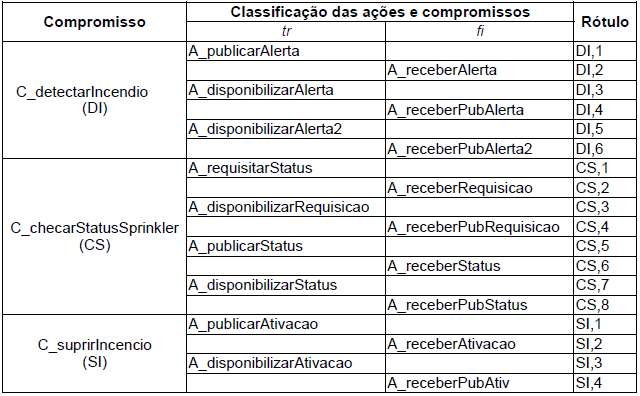
\includegraphics[width=9cm]{./figuras/tabela_estudo.png}
\end{figure} 
\end{frame}

\begin{frame}{Estudo de caso - Grafo de compromisso}
\begin{figure}[ht]
	\centering
	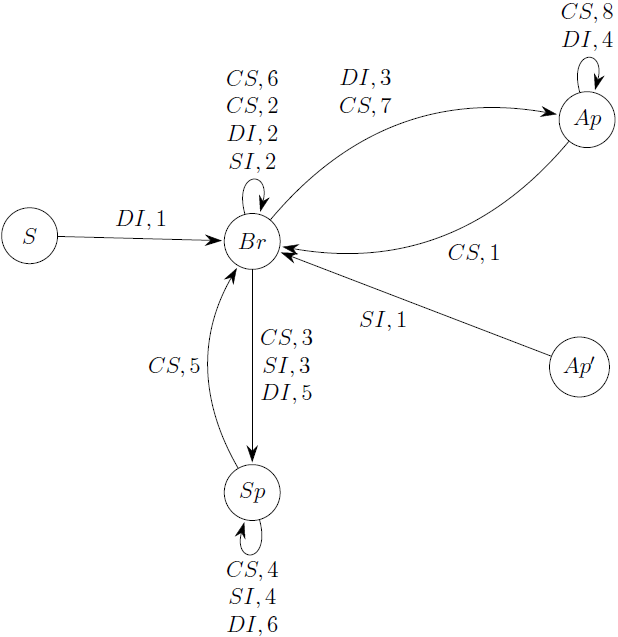
\includegraphics[width=6cm]{./figuras/estudo_grafo.png}
\end{figure} 
$ordercommitment = \{ (m_{2}), (m_{1} \cdot m_{2}), (m_{1} \cdot m_{2} \cdot m_{3}) \}$
\end{frame}

\begin{frame}{Estudo de caso - Cenário da violação}
	\begin{itemize}
		\item Um incêndio foi detectado pelo sensor;
		\item O aplicativo verificou que o status do \textit{sprinkler} consta como  \textbf{desativado};
		\item O compromisso de Supressão é disparado;
		\item Porém, o \textit{sprinkler} continua \textbf{desativado}.
	\end{itemize}
\end{frame}

\subsection{Aplicação do algoritmo}
\begin{frame}{Estudo de caso - Aplicação do algoritmo}
\begin{enumerate}
	\item Entradas:
		\begin{itemize}
			\item Contrato;
			\item Ação perdida: $a_{miss} = A\_receberAtivacao(SI_{2})$
			\item Última ação feita: $a_{done} = A\_publicarAtivacao(SI_{1})$
		\end{itemize}
	\item Localizar todas as ações que \textbf{não ocorreram} após a violação;
	$$E_{not\_occur} = \{SI_{3}, SI_{4}\}$$
	\item Encontrar todas as ações que \textbf{ocorreram} antes da violação;
	\begin{align}
	& E_{cut} = \{ DI_{1}, DI_{2}, DI_{3}, DI_{4}, DI_{5}, DI_{6}, CS_{1}, CS_{2}, \nonumber \\
	& CS_{3}, CS_{4}, CS_{5}, CS_{6}, CS_{7}, CS_{8} \}\nonumber
	\end{align}
	\item Montar o grafo restruturado.
\end{enumerate}
\end{frame}

\begin{frame}{Estudo de caso - Grafo restruturado}
\begin{figure}[ht]
	\centering
	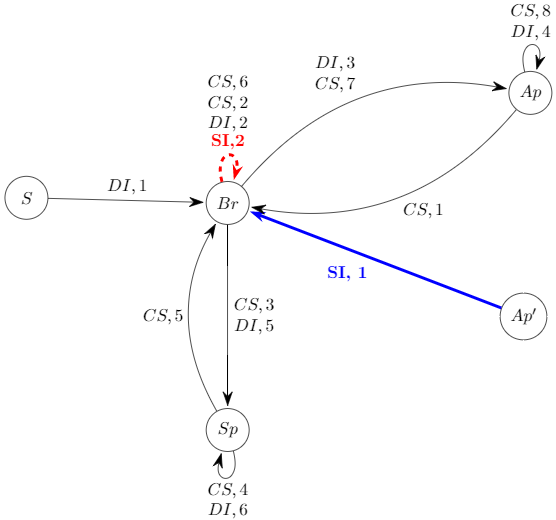
\includegraphics[width=7.7cm]{./figuras/grafo_final.png}
\end{figure}
\end{frame}

\begin{frame}{Estudo de caso - Detecção do responsável}
\begin{itemize}
	\item Se a mensagem \textit{"StartSprinkler"} enviada por $Ap'$ ao $Br$ ($SI, 1$) estiver incorreta, então $\textbf{Ap'}$ é o responsável;  
\end{itemize}
\begin{figure}[ht]
	\centering
	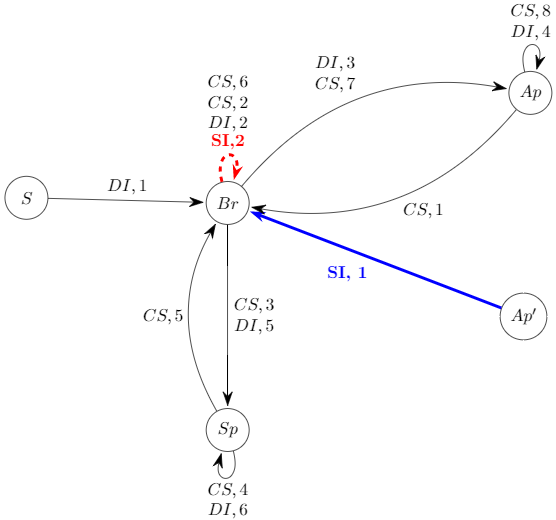
\includegraphics[width=6cm]{./figuras/grafo_final.png}
\end{figure}
\end{frame}

\begin{frame}{Estudo de caso - Detecção do responsável}
\begin{itemize}
	\item Caso contrário, a mensagem direcionada por $Br$ ao $Sp$ é verificada; 
	\item Se estiver incorreta, então $\textbf{Br}$ é o responsável;
\end{itemize}
\begin{figure}[ht]
	\centering
	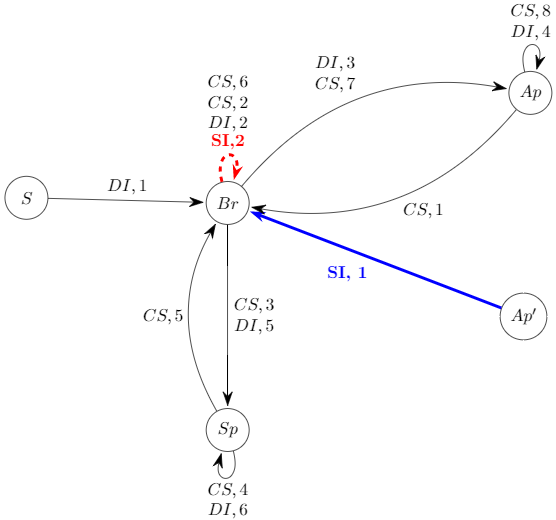
\includegraphics[width=6cm]{./figuras/grafo_final.png}
\end{figure}
\end{frame}

\begin{frame}{Estudo de caso - Detecção do responsável}
\begin{itemize}
	\item Se não, o responsável é o papel $\textbf{Sp}$.  
\end{itemize}
\begin{figure}[ht]
	\centering
	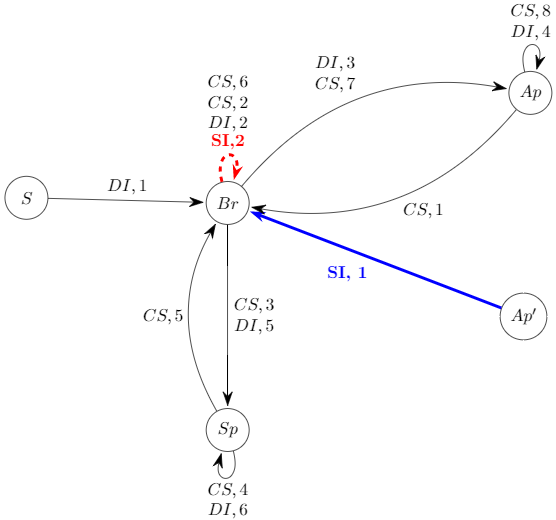
\includegraphics[width=6cm]{./figuras/grafo_final.png}
\end{figure}
\end{frame}

\section{Conclusão}
\begin{frame}{Conclusão}
\begin{itemize}
	\item Proposta: método para monitoramento reativo de protocolos IoT sobre o MQTT;
	\item É importante que violações sejam detectadas, assim como localizar o responsável;
	\item A solução proposta consiste em:
		\begin{enumerate}
			\item Descrever o modelo por meio do TPi;
			\item Desenvolver um método de conversão para representação em contrato multilateral;
			\item Aplicar o algoritmo de monitoramento;
		\end{enumerate}
	\item O que foi feito: 
		\begin{enumerate}
			\item Aplicação da proposta para comunicação QoS 0.
		\end{enumerate}
\end{itemize}
\end{frame}

\begin{frame}{Conclusão}
	\begin{itemize}
		\item Questões pendentes:
			\begin{enumerate}
				\item Representação em TPi dos papéis, suas propriedades;
				\item Representação das ordens de execução dos compromissos;
			\end{enumerate}
	\end{itemize}
	Trabalhos futuros:
	\begin{itemize}
		\item Determinar meios para representação em TPi das propriedades pendentes;
		\item Adaptar o método de conversão para casos mais complexos;
		\item Estender o método proposto para os níveis 1 e 2 de QoS;
		\item Desenvolver um \textbf{broker} MQTT para implemente o monitoramento reativo.
	\end{itemize}
\end{frame}

\frame{\titlepage}

\begin{frame}{QoS Níveis 1 e 2}
	\begin{figure}[ht]
		\centering
		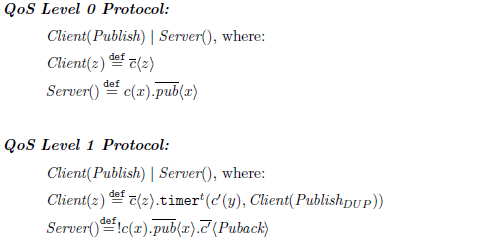
\includegraphics[width=8cm]{./figuras/mqtt_model.png}
	\end{figure}
\end{frame}

\begin{frame}{Sintaxe do TPi}
		\begin{figure}[ht]
		\centering
		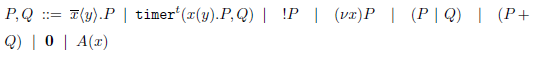
\includegraphics[width=8cm]{./figuras/tpi_syntax.png}
	\end{figure}
\end{frame}

%
\begin{frame}
    \vfill
    \centering
    \begin{beamercolorbox}[sep=8pt,center,shadow=true,rounded=true]{title}
        \usebeamerfont{title}Adicionais
    \end{beamercolorbox}
    \vfill
\end{frame}

\section{Fundamentação Teórica}

\subsection{Lógica Deôntica}
\begin{frame}{Lógica Deôntica}
    \begin{itemize}
        \item A Lógica Deôntica Padrão (SDL) é a variação mais utilizada.
        \item Representa conceitos normativos legais e éticos.
        \item Uma norma pode definir direitos, deveres, e proibições.
        \item As normas podem ser:
        \begin{enumerate}
            \item Obrigação de executar uma ação - $O(\alpha)$.
            \item Permissão para executar uma ação - $P(\alpha)$.
            \item Proibição para executar uma ação - $F(\alpha)$.
        \end{enumerate}
    \end{itemize}
\end{frame}

\section{Trabalhos Relacionados}
%\subsection{Detecção de conflitos - Fenech}
%\begin{frame}{Algoritmo para detecção de conflitos}
%	O algoritmo consiste nas seguintes etapas:
%	\begin{itemize}
%		\item Criação de um autômato que representa o contrato
%		\begin{enumerate}
%			\item O estado inicial representa o contrato completo
%			\item São criadas transições com todas as ações possíveis
%			\item O autômato possui dois estados importantes: {\color{red}$V$} e {\color{OliveGreen}$Sat$}
%		\end{enumerate}
%		\item Busca por conflitos nos estados do autômato
%		\begin{enumerate}
%			\item Cada estado contém \textbf{informações deônticas} do contrato
%			\item Caso exista conflito entre essas informações, \textbf{o contrato está em conflito}
%		\end{enumerate}
%	\end{itemize}
%	
%\end{frame}
%
%\begin{frame}{Exemplo do Algoritmo}
%	\begin{block}{}
%		Considere o contrato $[a]O(b) \wedge [b]F(b)$ e o autômato resultante:
%	\end{block}
%	\begin{figure}[ht]
%		\centering
%		\includegraphics[width=6cm]{./figuras/exemplo}
%	\end{figure}
%\end{frame}

\subsection{Lógica Deôntica Relativizada}

\begin{frame}{Lógica Deôntica Relativizada}
	\begin{itemize}
		\item Na SDL as expressões são escritas sem revelar os indivíduos.
		\item A expressão $O(a)$ não indica quem deve executar a ação.
		\item Esta impessoalidade torna limitada o uso da SDL em contratos.
		\item A \textbf{Lógica Deôntica Relativizada}, representa qual indivíduo está presente na sentença.
		\item A relativização pode gerar:
		\begin{enumerate}
			\item Obrigação pessoal
			\item Obrigação geral
			\item Obrigação impessoal
			\item Obrigação direcionada
		\end{enumerate}
	\end{itemize}
\end{frame}

\begin{frame}{Lógica Deôntica Relativizada - Herrestad e Krogh}
    \begin{itemize}
        \item Na SDL as expressões são escritas sem revelar os indivíduos (limita seu uso em contratos).
        \item A expressão $O(\alpha)$ não indica quem deve executar a ação.
        \item A \textbf{Lógica Deôntica Relativizada}, representa qual indivíduo está presente na sentença (identificados por $i \in I$).
        \item A sentença $_iO(\alpha)$ indica que $i$ é obrigado a executar a ação $\alpha$.
        \item \textbf{Operadores Relativizados:} $_iO(\alpha), \ _iP(\alpha), \ _iF(\alpha)$.
        \item A fórmula $_iO_j(\alpha)$ expressa que $i$ é obrigado a executar a ação $\alpha$ para $j$, com $i,j \in I$ (Executor e Recebedor da ação).
        \item \textbf{Operadores Direcionados:} $_iO_j(\alpha), \ _iP_j(\alpha), \ _iF_j(\alpha)$.
        \item \textbf{Modalidade Geral:} $O(\alpha) \iff \forall i \in I \ _iO(\alpha)$.
    \end{itemize}
\end{frame}

\begin{frame}{Operadores deônticos relativizados}
	\begin{itemize}
		\item Nesta abordagem os indivíduos são identificados por $i \in I$.
		\item A sentença $_iO(a)$ indica que o indivíduo $i$ é obrigado a executar a ação $a$.
		\item O mesmo ocorre com:
		\begin{itemize}
			\item Permissão relativizada: $_iP(a) \equiv \neg \mbox{ } _iO(\neg a)$ 
			\item Proibição relativizada: $_iF(a) \equiv \mbox{ } _iO(\neg a)$.
		\end{itemize} 
		\item Obrigação e permissão geral: $\forall i \in I\mbox{ }_iO(p) \mbox{ e } \forall i \in I\mbox{ }_iP(p)$;
		\item Obrigação e permissão impessoal: $\exists i \in I\mbox{ }_iO(p) \mbox{ e } \exists i \in I\mbox{ }_iP(p)$.
	\end{itemize}
\end{frame}

\begin{frame}{Operadores deônticos direcionados}
	\begin{itemize}
		\item Em certos contratos é importante definir o portador da obrigação e o requerente (ou contra-parte).
		\item Indicar o responsável pela ação e quem vai receber esta ação.
		\item A fórmula $_iO_j(a)$ expressa que $i$ é obrigado a executar a ação $a$ para $j$, tal que $i,j \in I$.
	\end{itemize}
\end{frame}

\begin{frame}{Sintaxe da $\mathcal{CL}$}
    \begin{itemize}
        \item As expressões são baseadas em \textbf{ações atômicas}.
        \item Os indivíduos são incorporados apenas nas ações e \underline{não podem ser representados pela linguagem}.
    \end{itemize}
    \begin{block}{A sintaxe da linguagem}
        \centering
        \begin{tabular}{rll}
            $\mathcal{C}$ & $:=$ & $\phi \mid O_\mathcal{C}(\alpha) \mid P(\alpha) \mid F_\mathcal{C}(\alpha) \mid \mathcal{C} \to \mathcal{C} \mid [\delta]\mathcal{C} \mid \perp $\\
            $\alpha$ & $:=$ & $ a \mid \textbf{0} \mid \textbf{1} \mid \alpha \times \alpha \mid \alpha \cdot \alpha \mid \alpha + \alpha$ \\
            $\delta$ & $:=$ & $ a \mid \textbf{0} \mid \textbf{1} \mid \delta \times \delta \mid \delta \cdot \delta \mid \delta + \delta \mid \delta^* \mid \varphi?$ \\
            $\varphi$ & $:=$ & $ \phi \mid \textbf{0} \mid \textbf{1} \mid \varphi \vee \varphi \mid \varphi \wedge \varphi \mid \neg \varphi$ \\
        \end{tabular}
    \end{block}
\end{frame}

\begin{frame}{Semântica da $\mathcal{CL}$}
\begin{itemize}
\item Semântica de \textit{traces}: sequência de ações que respeita o contrato
\item Um \textit{trace} $\sigma$ é uma sequência ordenada de ações
 dada por $a_0, a_1, \dots$, onde $a_i \in \mathcal{A}^\&_\mathcal{B}$, $i\geq 0$.
\item Se o \textit{trace} $\sigma$ satisfaz contrato $\mathcal{C}$, então  $\sigma \models \mathcal{C}$
\item Se o \textit{trace} $\sigma$ viola o contrato, então $\sigma \not \models \mathcal{C}$
\end{itemize}

\begin{block}{Exemplo}
\begin{center}
{\footnotesize 
Se o cliente exceder o limite de banda da internet ele deve pagar uma multa, ou 
 deve atrasar o pagamento e notificar o provedor. Senão, ele paga o dobro.
 }
\end{center}
$$ \mathcal{C} = [exceder]O_{O_{\perp}(pagar\cdot pagar)}(pagar + atrasar \times notificar)$$ 
$$ \sigma = \langle exceder, atrasar, pagar\cdot pagar \rangle $$
\end{block}
\end{frame}

\begin{frame}{Semântica para detecção de conflitos}
\begin{itemize}
\item A semântica (de \textit{traces}) descreve quais condições respeitam os operadores da $\mathcal{CL}$.
\item $\sigma$ é uma \textbf{sequência de ações} que satisfazem o contrato
\item $\sigma_d$ contém as \textbf{informações deônticas do contrato} 
\item Seja $\mathcal{C} = [a]O(b)\wedge[b]F(b)$, um dos \textit{traces} que satisfazem $\mathcal{C}$:
$$\sigma = [\{a\}, \{b\}, \{b\}]$$
$$\sigma_d = [\ \emptyset\ , \{O_b\},\ \emptyset \ ]$$
\item Esta situação pode ser representada por $\sigma,\sigma_d\models\mathcal{C}$.
\item Os \textit{traces} levam a uma situação de conflito:
\[\sigma = [\{a\times b\},\emptyset,\emptyset]\] 
\[\sigma_d = [\emptyset, \{\{O_b\},\{F_b\}\},\emptyset]\]
\item Levam a uma situação onde não é possível satisfazer o contrato.
\end{itemize}
\end{frame}

\begin{frame}{Algoritmo para detecção de conflitos}
O algoritmo consiste nas seguintes etapas:
\begin{itemize}
\item Criação de um autômato que representa o contrato
	\begin{enumerate}
	\item O estado inicial representa o contrato completo
	\item São criadas transições com todas as ações possíveis
	\item O autômato possui dois estados importantes: {\color{red}$V$} e {\color{OliveGreen}$Sat$}
	\end{enumerate}
\item Busca por conflitos nos estados do autômato
	\begin{enumerate}
	\item Cada estado contém \textbf{informações deônticas} do contrato
	\item Caso exista conflito entre essas informações, \textbf{o contrato está em conflito}
	\end{enumerate}
\end{itemize}

\end{frame}

\begin{frame}{Algoritmo para detecção de conflitos}
\begin{block}{}
Considere o contrato $[a]O(b) \wedge [b]F(b)$ e o autômato resultante:
\end{block}
\begin{figure}[ht]
\centering
\includegraphics[width=6cm]{./figuras/exemplo}
\end{figure}
\end{frame}




\section{Método proposto}


\begin{frame}{Sintaxe da $\mathcal{RCL}$}
    \begin{block}{}
        \centering
        \begin{tabular}{l}
            $\mathcal{C}::=\mathcal{C}_O \mid \mathcal{C}_P \mid \mathcal{C}_F \mid \mathcal{C} \wedge \mathcal{C} \mid \mathcal{C}_D\mid\top \mid\  \perp$\\\quad\\
            $\mathcal{C}_O::= O_\mathcal{C}(\alpha) \mid\ _iO_\mathcal{C}(\alpha) \mid \ _{i \curvearrowright  j}O_\mathcal{C}(\alpha) \mid \mathcal{C}_O \oplus \mathcal{C}_O$\\
            $\mathcal{C}_P::= P(\alpha) \mid \ _iP(\alpha) \mid \ _{i \curvearrowright  j}P(\alpha) \mid \mathcal{C}_P \oplus \mathcal{C}_P$\\
            $\mathcal{C}_F::=F_\mathcal{C}(\alpha) \mid \ _iF_\mathcal{C}(\alpha) \mid \ _{i \curvearrowright  j}F_\mathcal{C}(\alpha) \mid \mathcal{C}_F \vee \mathcal{C}_D \mathcal{C}_F$\\
            $\mathcal{C}_D ::=[\beta]\mathcal{C} \mid \ _i[\beta]\mathcal{C} \mid \ _{i \curvearrowright  j}[\beta]\mathcal{C}_D$\\\quad\\
            $\alpha::= 0 \mid 1 \mid a \mid \alpha \times \alpha \mid \alpha \cdot \alpha \mid \alpha + \alpha$\\
            $\beta::=  0 \mid 1 \mid a \mid \beta \times \beta \mid \beta \cdot \beta \mid \beta + \beta \mid \overline{\beta}  \mid \beta^*$
        \end{tabular}
    \end{block}
\end{frame}



%\begin{frame}{Semântica $\mathcal{RCL}$}
%    \begin{itemize}
%        \item \textit{Trace}: \textbf{sequência de ações} executadas no contrato.
%        \item A semântica é baseada em  \textbf{\textit{trace} de ações} e \textbf{\textit{trace} deôntico}
%        \item Ação Relativizada: $a_r = \langle i, \alpha, j\rangle$
%        \item Todas as ações: $\mathcal{A}_r = \{\mathcal{I} \times \mathcal{A_B} \times \mathcal{I}\}$\\
%        \item Representações deônticas: $\mathcal{M} = \{O_{\alpha},\  _{i}O_{\alpha},\ _{j\curvearrowright i}O_{\alpha},\dots\}$
%        
%        \item A semântica é baseada em dois \textit{traces}:
%        \begin{itemize}
%            \item \textit{trace} de ações ($\sigma: \mathbb{N} \to 2^{\mathcal{A}_r}$)
%            \item \textit{trace} deôntico ($\sigma_d: \mathbb{N} \to 2^\mathcal{M}$)
%        \end{itemize}
%    \end{itemize}
%    \begin{block}{Exemplo}
%        $\mathcal{C} =\ _{c \curvearrowright v}O(pagar)\ \wedge\ _{c \curvearrowright v}[pagar]\ _{v \curvearrowright c}O(entregar)$
%        
%        \begin{itemize}
%            \item $\sigma = \langle \{(c,pagar,v)\}, \{(v,entregar,c)\}\rangle$
%            \item $\sigma_d = \langle\{_{c\curvearrowright v}O_{pagar} \}, \{_{v\curvearrowright c}O_{entregar} \} \rangle$
%        \end{itemize}
%    \end{block}
%\end{frame}
%
%\begin{frame}{Semântica Relativizada da $\mathcal{CL}$ - Satisfação}
%    \begin{itemize}
%        \item Definir  $\sigma, \sigma_d \models \mathcal{C}$, ou seja, se o \textit{trace} se ações $\sigma$ e o \textit{trace} deôntico $\sigma_d$ satisfazem o contrato $\mathcal{C}$.
%    \end{itemize}
%    
%    \quad
%    
%    \centering
%    $\sigma,\sigma_d \models _{i\curvearrowright j}O_\mathcal{C}(\alpha)$ se {\color{purple}$_{i\curvearrowright j}O_{\alpha}\in\sigma_d(0)$} e \\
%    ({\color{blue}$(\exists \varphi \in \sigma(0) \mid \varphi = \langle i, \alpha, j \rangle \mbox{ e } \sigma(1\dots),\sigma_d(1\dots) \models \top)$} \\
%    ou  {\color{red} $(\sigma(1\dots),\sigma_d(1\dots) \models \mathcal{C})$ })
%\end{frame}


\subsection{Semântica Relativizada}
    \begin{frame}{Semântica Relativizada da $\mathcal{CL}$}
        \begin{itemize}
            \item A semântica proposta para a nova sintaxe é baseada em \textit{traces} que representam as ações executadas no contrato.
        \end{itemize}
        \begin{block}{Ação Relativizada}
            \begin{itemize}
                \item Uma tupla $a_r = \langle\kappa,\chi,\lambda\rangle \mid \kappa,\lambda \in \mathcal{I}$ e $\chi \in \mathcal{A_B}$
                \item Ações relativizadas: $\mathcal{A}_r = \{\mathcal{I} \times \mathcal{A_B} \times \mathcal{I}\}$\\
            \end{itemize}
        \end{block}
        \begin{itemize}
            \item Representações deônticas: $\mathcal{M} = \{_rd_\alpha \mid r\in \mathcal{R}, d \in \mathcal{D}, \alpha \in \mathcal{A_B} \}$
            \item A semântica é baseada em dois \textit{traces}:
            \begin{enumerate}
                \item \textit{trace} de ações: denotado por $\sigma: \mathbb{N} \to \mathcal{A}^2_r$
                \item \textit{trace} deôntico: denotado por $\sigma_d: \mathbb{N} \to 2^\mathcal{M}$
            \end{enumerate}
        \end{itemize}
    \end{frame}
    
    \begin{frame}{Semântica Relativizada da $\mathcal{CL}$ - \textit{Traces}}
        \begin{enumerate}
            \item A modalidade global $O(\alpha)$ gera $\sigma(0) \subseteq \{\langle x ,\alpha, y\rangle \mid y \in \mathcal{I}, \forall x \in \mathcal{I}\}$.
            \item A modalidade relativizada $_{i}O(\alpha)$ gera $\sigma(0) \subseteq \{\langle i,\alpha, x\rangle \mid x \in \mathcal{I}\}$.
            \item A modalidade direcionada $_{i\curvearrowright j}O(\alpha)$ gera $\sigma(0) \subseteq \{\langle i,\alpha,j\rangle \mid i,j \in \mathcal{I}\}$.
        \end{enumerate}
        Seja o contrato: $\mathcal{C} =\ _{i \curvearrowright j}O(pagar)\ \wedge\ _{i \curvearrowright j}[pagar]\ _{j \curvearrowright i}O(entregar)$
        \\$\quad$\\
        \textbf{Os \textit{traces} que podem satisfazer o contrato são:}
        \begin{itemize}
            \item $\sigma = \langle \{(i,pagar,j)\}, \{(j,entregar,i)\}\rangle$
            \item $\sigma_d = \langle\{_{i\curvearrowright j}O_{pagar} \}, \{_{j\curvearrowright i}O_{entregar} \} \rangle$
        \end{itemize}
    \end{frame}
    
    \begin{frame}{Semântica Relativizada da $\mathcal{CL}$ - Satisfação}
        \begin{itemize}
            \item Definir  $\sigma, \sigma_d \models \mathcal{C}$, ou seja, se o \textit{trace} se ações $\sigma$ e o \textit{trace} deôntico $\sigma_d$ satisfazem o contrato $\mathcal{C}$.
        \end{itemize}
        
        {\small 
            $\sigma,\sigma_d \models O_\mathcal{C}(\alpha)$ se {\color{purple}$O_{\alpha} \in \sigma_d(0) $} e \\
            ({\color{blue}$(\forall i \in \mathcal{I}, \exists \varphi \in \sigma(0), x \in \mathcal{I} \mid \varphi = \langle i, \alpha, x\rangle \mbox{ e } \sigma(1\dots),\sigma_d(1\dots) \models \top)$} \\
            ou  {\color{red} $(\sigma(1\dots),\sigma_d(1\dots) \models \mathcal{C})$})
            \\\quad\\
            $\sigma,\sigma_d \models _iO_\mathcal{C}(\alpha)$ se {\color{purple}$_iO_{\alpha}\in\sigma_d(0) $} e \\
            ({\color{blue}$(\exists \varphi \in \sigma(0), x\in \mathcal{I} \mid \varphi = \langle i,\alpha,x\rangle  \mbox{ e } \sigma(1\dots),\sigma_d(1\dots) \models \top)$} \\
            ou  {\color{red} $(\sigma(1\dots),\sigma_d(1\dots) \models \mathcal{C})$ })
            \\\quad\\
            $\sigma,\sigma_d \models _{i\curvearrowright j}O_\mathcal{C}(\alpha)$ se {\color{purple}$_{i\curvearrowright j}O_{\alpha}\in\sigma_d(0)$} e \\
            ({\color{blue}$(\exists \varphi \in \sigma(0) \mid \varphi = \langle i, \alpha, j \rangle \mbox{ e } \sigma(1\dots),\sigma_d(1\dots) \models \top)$} \\
            ou  {\color{red} $(\sigma(1\dots),\sigma_d(1\dots) \models \mathcal{C})$ })
        }
    \end{frame}
    
\subsection{Construção do Autômato}    
    \begin{frame}{Construção do autômato}
        \begin{block}{Visão Geral}
            O processo de detecção de conflitos proposto consiste na construção do autômato que representa os \textit{traces} que satisfazem o contrato.
        \end{block}
        \centering$\mathcal{A}(\mathcal{C})= \langle S, \mathcal{A}^2_r, \mathcal{M}, \mathcal{I}, s_0, T, V, l, \delta \rangle$
        
        \begin{itemize}
            \item $S$: conjunto de estados do autômato;
            \item $\mathcal{A}^2_r$: conjunto de ações relativizadas concorrentes;
            \item $\mathcal{M}$: conjunto de rótulos deônticos;
            \item $\mathcal{I}$: conjunto de indivíduos;
            \item $s_0$: estado inicial;
            \item $T \subseteq S \times \mathcal{A}^2_r \times S$: relação de transições rotuladas;
            \item $V$: estado de violação do contrato;
            \item $l : S \to \mathcal{C}$ rotula os estados com contratos decompostos; e
            \item  $\delta: S \to 2^{\mathcal{M}}$ rotula os estados com informações deônticas.
        \end{itemize}
    \end{frame}
    
    \begin{frame}{Algoritmo de construção do Autômato}
        \centering\scalebox{.7}{
            \begin{algorithm}[H]
                \SetKwFunction{construirAutomato}{construirAutomato}
                \SetKwFunction{buscarConflitos}{buscarConflitos}
                \SetKwInOut{Input}{input}\SetKwInOut{Output}{output}
                \uIf{\buscarConflitos(s)}{
                    um conflito foi encontrado no estado $s$\;
                }\uElseIf{$l(s) = \top$}{
                $T \gets T \cup (s,\top,s)$\;
            }\uElseIf{$l(s) = \bot$}{
            $V \gets s$\;
            $T \gets T \cup (V,\perp,V)$\;
        }\Else{
        \For{$\alpha \in \mathcal{A}^2_r$}{
            $\mathcal{C}'\gets f(l(s),\alpha)$\;
            \uIf{$\exists s' \in S \mid l(s') = \mathcal{C}'$}{
                $T \gets T \cup (s,\alpha,s')$\;
            }\Else{
            $S \gets S \cup s'$\;
            $l(s') \gets \mathcal{C}'$\;	
            $T \gets T \cup (s,\alpha,s')$\;
            $\delta(s') \gets f_d(\mathcal{C}')$\;
            \construirAutomato($s'$)\;
        }
    }
}
\end{algorithm}
}
\end{frame}

\subsection{Detecção de Conflitos}
\begin{frame}{Detecção de Conflitos}
    Os conflito tratados pelo algoritmo são caracterizados por:
    \begin{enumerate}
        \item uma ação entre operadores deônticos de obrigação e proibição;
        \item uma ação entre operadores deônticos de proibição e permissão;
        \item ações conflitantes entre operadores de obrigação; 
        \item ações conflitantes entre permissão e obrigação. 
    \end{enumerate} 
    
    \begin{itemize}
        \item \textbf{Sem conflitos:} Operadores relativizados associados a uma mesma ação executada por indivíduos distintos: {\color{blue}$_iO(\alpha) \wedge\ _jF(\alpha)$}
        \item \textbf{Sempre em conflito:} Um operador global deôntico de obrigação sempre está em conflito com os operadores relativizados de proibição: {\color{red}$O(\alpha) \wedge\ _iF(\alpha)$}
        $$O(\alpha) \iff \forall x \in \mathcal{I}, \ _xO_\mathcal{C}(\alpha) \wedge\ _iF(\alpha)$$
    \end{itemize}
\end{frame}

\begin{frame}{Relação de Conflito}
    A relação de conflito é denotada por $\# \subseteq \mathcal{A}_r \times  \mathcal{A}_r$
    \begin{itemize}
        \item Determina que duas ações relativizadas não podem ocorrer ao mesmo tempo.
        \item Possui duas formas: 
        \begin{enumerate}
            \item \textbf{relação de conflito global}, denotada por $\#_g \subseteq \mathcal{A_B} \times \mathcal{A_B}$, indica que as duas ações não podem ocorrer ao mesmo tempo independente do indivíduo executor. 
            $$\alpha\#_g\ \beta \iff \forall i,j \in \mathcal{I}, \langle i, \alpha, x\rangle \# \langle j, \beta, y\rangle \text{ com } x,y \in \mathcal{I}$$
            
            \item \textbf{relação de conflito relativizada}, denotada por $\#_r \subseteq \mathcal{A_B} \times \mathcal{A_B}$, indica que as duas ações não podem ser executadas ao mesmo tempo por um mesmo indivíduo executor.
            $$\alpha\#_r\ \beta \iff \forall i \in \mathcal{I}, \langle i, \alpha, x\rangle \# \langle i, \beta, y\rangle \text{ com } x,y \in \mathcal{I}$$
        \end{enumerate}
    \end{itemize}
\end{frame}

\begin{frame}{Algoritmo de Busca por Conflitos}
    \begin{itemize}
        \item Para cada estado criado pelo algoritmo de construção
        \item É realizada uma busca por conflitos no contrato resultante
    \end{itemize}	
    
    \centering\scalebox{.6}{
        \begin{algorithm}[H]
            \SetKwInOut{Input}{input}\SetKwInOut{Output}{output}
            \Input{Um estado $s$ do autômato $\mathcal{A(C)}$}
            \Output{Uma situação de conflito.}
            \Begin{
                \For{$\mathcal{D}\in\delta(s)$}{
                    \For{$\mathcal{D}' \in \delta(s)-\{\mathcal{D}\}$}{
                        \If{$\exists d \in \mathcal{D} \mid f_\#(d)\cap \mathcal{D}' \neq \emptyset$}{
                            \Return Conflito entre $d$ e $f_\#(d)\cap \mathcal{D}'$\;
                        }
                    }
                }
                \Return Nenhum Conflito\;
            }
        \end{algorithm}
    }
    \begin{itemize}
        \item A função $\delta(s)$ retorna os marcadores deônticos do estado $s$
        \item A função $f_\#(d)$ retorna os marcadores que conflitam com $d$
    \end{itemize}
\end{frame}

\subsection{Exemplo}
\begin{frame}{Exemplo}
    \begin{block}{Contrato em \CL}
        $$\mathcal{C} =\ _{i\curvearrowright j}[a]\ _{j_\curvearrowright i}O(b) \wedge \ _{j\curvearrowright i}[b]\ _{j\curvearrowright i}F(b)$$
    \end{block}
    
    \begin{itemize}
        \item Sejam
        \begin{itemize}
            \item Indivíduos: $i$ (cliente) e $j$ (vendedor)
            \item Ações: $a$ (pagar) e $b$ (entregar o produto)
        \end{itemize}
        
        \begin{block}{Contrato}
            \begin{itemize}
                \item Após o \underline{cliente} \textbf{pagar} o \underline{vendedor}, \\ o \underline{vendedor} é obrigado a \textbf{entregar o produto} para o \underline{cliente}
                \item Após o \underline{vendedor} \textbf{entregar o produto} para o \underline{cliente}, \\ o \underline{vendedor} é proibido \textbf{entregar o produto} para o \underline{cliente}
            \end{itemize}
        \end{block}
    \end{itemize}
\end{frame}

\begin{frame}{Exemplo - Fenech x Proposta}
    \begin{columns}[onlytextwidth]
        \begin{column}{0.48\textwidth}
            \begin{block}{Método de Fenech}
                {\small$\mathcal{C} = [a]O(b) \wedge [b]F(b)$}
                
                \quad
                
                Após ({\color{red}alguém}) \textbf{pagar} ({\color{red}quem?}), é obrigado \textbf{entregar} ({\color{red}quem entrega para quem?}).
                
                \quad
                
                \quad
                
                Após ({\color{red}alguém}) \textbf{entregar}, é proibido ({\color{red}alguém}) \textbf{entregar}.
                
                \quad
                
                \quad
                
                \quad
                
            \end{block}
        \end{column}
        \begin{column}{0.48\textwidth}
            \begin{block}{Método Proposto}
                {\small $\mathcal{C} =\ _{i\curvearrowright j}[a]\ _{j_\curvearrowright i}O(b) \wedge \ _{j\curvearrowright i}[b]\ _{j\curvearrowright i}F(b)$}
                
                \quad
                
                Após o \underline{cliente} \textbf{pagar} o \underline{vendedor}, \\ o \underline{vendedor} é obrigado a \textbf{entregar} para o \underline{cliente}.
                
                \quad
                
                \quad
                
                Após o \underline{vendedor} \textbf{entregar} para o \underline{cliente}, \\ o \underline{vendedor} é proibido \textbf{entregar} para o \underline{cliente}.
                
                \quad
                
            \end{block}
        \end{column}
    \end{columns}
\end{frame}

\begin{frame}{Exemplo - Aplicação}
    \begin{columns}[onlytextwidth]
        \begin{column}{0.6\textwidth}
            \scalebox{.6}{
                \begin{tikzpicture}[->,>=stealth,shorten >=1pt,auto,node distance=4cm,initial text={},semithick]
                \tikzstyle{every state}=[text=black]
                \tikzstyle{conflict}=[draw=black!100,fill=black!20,text=black]
                \tikzstyle{conflict-label}=[draw=black!100,fill=black!10,text=black]
                \tikzstyle{contract}=[fill = gray!20, shape = rectangle, rounded corners, font = \sffamily]
                
                \node[initial,state] 		   (s_0)          	{$s_0$};
                \node[contract] at (0,1) (s_0-cl)	{{\small $\ _{i\curvearrowright j}[a]\ _{j\curvearrowright i}O(b) \wedge \ _{j \curvearrowright i}[b]\ _{j\curvearrowright i}F(b)$}};
                
                \node[state]         (s_1) [below left of=s_0] 	{$s_1$};
                \node[contract] at (-4.5,-2.5) (s_1-cl)	{{\small $\ _{j\curvearrowright i}O(b)$}};
                \node[state]         (s_2) [below  of=s_0] 	{$s_2$};
                \node[contract] at (1.5,-4.1) (s_2-cl)	{{\small $\ _{j\curvearrowright i}F(b)$}};
                \node[state, conflict]         (s_3) [right of=s_2] 	{$s_3$};
                \node[contract, conflict-label] at (4,-5) (s_3-cl)	{\textbf{{\small $\ _{j\curvearrowright i}O(b)\wedge\ _{j\curvearrowright i}F(b) $}}};  
                
                \node[state] (s_4) [below left of=s_1,yshift=-2cm] 	{$s_4$};
                \node[contract] at (-7,-8) (s_4-cl)	{$SAT$};  
                \node[state] (s_5) [below right of=s_2,yshift=-2cm] 	{$s_5$};
                \node[contract] at (4,-9) (s_5-cl)	{$V$};
                
                \path (s_0)	edge	[bend right] 	node[left] 								{{\tiny 1,5,6,11}} (s_1);
                \path (s_0)	edge	 			 	node[right] 							{{\tiny 4,9,10,14}} (s_2);
                \path (s_0)	edge	[bend left] 	node	 								{{\tiny 7,12,14,15}} (s_3);
                \path (s_0)	edge					node[right,xshift=-0.5cm,yshift=-1cm]	{{\tiny 2,3,8}} (s_4);  
                \path (s_1)	edge	[bend right] 	node[left]								{{\tiny 4,7,9,10,12,13,14,15}} (s_4);
                \path (s_1)	edge	[bend right] 	node[right,xshift=0.2cm]	{{\tiny 1,2,3,5,6,8,11}} (s_5);  
                \path (s_2)	edge	[bend left] 	node[right,xshift=-1cm,yshift=-0.7cm]				{{\tiny 1,5,6,7,11,12,13,15}} (s_4);
                \path (s_2)	edge			 	node[right,yshift=-0.5cm,xshift=0.2cm]	{{\tiny 2,3,4,8,9,10,14}} (s_5);
                \end{tikzpicture}
            }
        \end{column}
        \begin{column}{0.3\textwidth}
            \begin{table}[H]
                \centering \tiny{
                    \begin{tabular}{|p{1pt}|l|}
                        \hline \textbf{N} & \textbf{Ações Concorrentes} \\
                        \hline $1$ & $(i,a,j)$\\ 
                        \hline $2$ & $(i,b,j)$\\ 
                        \hline $3$ & $(j,a,i)$\\ 
                        \hline $4$ & $(j,b,i)$\\
                        \hline $5$ & $(i,a,j)\times(i,b,j)$\\ 
                        \hline $6$ & $(i,a,j)\times(j,a,i)$\\ 
                        \hline $7$ & $(i,a,j)\times(j,b,i)$\\ 
                        \hline $8$ & $(i,b,j)\times(j,a,i)$\\ 
                        \hline $9$ & $(i,b,j)\times(j,b,i)$\\ 
                        \hline $10$ & $(j,a,i)\times(j,b,i)$\\ 
                        \hline $11$ & $(i,a,j)\times(i,b,j)\times(j,a,i)$\\ 
                        \hline $12$ & $(i,a,j)\times(i,b,j)\times(j,b,i)$\\ 
                        \hline $13$ & $(i,a,j)\times(j,a,i)\times(j,b,i)$\\ 
                        \hline $14$ & $(i,b,j)\times(j,a,i)\times(j,b,i)$\\ 
                        \hline $15$ & $(i,a,j)\times(i,b,j)\times$\\&$(j,a,i)\times(j,b,i)$\\
                        \hline
                    \end{tabular}
                }
            \end{table}
        \end{column}
    \end{columns}
\end{frame}

\begin{frame}{Exemplo: Proposta x Fenech}
    \begin{columns}[onlytextwidth]
        \begin{column}{0.55\textwidth}
            \centering \small \textbf{Método Proposto}
            \scalebox{.5}{
                \begin{tikzpicture}[->,>=stealth,shorten >=1pt,auto,node distance=4cm,initial text={},semithick]
                \tikzstyle{every state}=[text=black]
                \tikzstyle{conflict}=[draw=black!100,fill=black!90,text=white]
                \tikzstyle{conflict-label}=[draw=black!100,fill=black!60,text=white]
                \tikzstyle{contract}=[fill = gray!20, shape = rectangle, rounded corners, font = \sffamily]
                
                \node[initial,state] 		   (s_0)          	{$s_0$};
                \node[contract] at (0,1) (s_0-cl)	{{\small $\ _{i\curvearrowright j}[a]\ _{j\curvearrowright i}O(b) \wedge \ _{j \curvearrowright i}[b]\ _{j\curvearrowright i}F(b)$}};
                
                \node[state]         (s_1) [below left of=s_0] 	{$s_1$};
                \node[contract] at (-4.5,-2.5) (s_1-cl)	{{\small $\ _{j\curvearrowright i}O(b)$}};
                \node[state]         (s_2) [below  of=s_0] 	{$s_2$};
                \node[contract] at (1.5,-4.1) (s_2-cl)	{{\small $\ _{j\curvearrowright i}F(b)$}};
                \node[state, conflict]         (s_3) [right of=s_2] 	{$s_3$};
                \node[contract, conflict-label] at (4,-5) (s_3-cl)	{\textbf{{\small $\ _{j\curvearrowright i}O(b)\wedge\ _{j\curvearrowright i}F(b) $}}};  
                
                \node[state] (s_4) [below left of=s_1,yshift=-2cm] 	{$s_4$};
                \node[contract] at (-7,-8) (s_4-cl)	{$SAT$};  
                \node[state] (s_5) [below right of=s_2,yshift=-2cm] 	{$s_5$};
                \node[contract] at (4,-9) (s_5-cl)	{$V$};
                
                \path (s_0)	edge	[bend right] 	node[left] 								{{\tiny 1,5,6,11}} (s_1);
                \path (s_0)	edge	 			 	node[right] 							{{\tiny 4,9,10,14}} (s_2);
                \path (s_0)	edge	[bend left] 	node	 								{{\tiny 7,12,14,15}} (s_3);
                \path (s_0)	edge					node[right,xshift=-0.5cm,yshift=-1cm]	{{\tiny 2,3,8}} (s_4);  
                \path (s_1)	edge	[bend right] 	node[left]								{{\tiny 4,7,9,10,12,13,14,15}} (s_4);
                \path (s_1)	edge	[bend right] 	node[right,xshift=0.2cm]	{{\tiny 1,2,3,5,6,8,11}} (s_5);  
                \path (s_2)	edge	[bend left] 	node[right,xshift=-1cm,yshift=-0.7cm]				{{\tiny 1,5,6,7,11,12,13,15}} (s_4);
                \path (s_2)	edge			 	node[right,yshift=-0.5cm,xshift=0.2cm]	{{\tiny 2,3,4,8,9,10,14}} (s_5);
                \end{tikzpicture}
            }
        \end{column}
        \begin{column}{0.45\textwidth}
            \centering \small \textbf{Método de Fenech}
            \begin{figure}[ht]
                \centering
                \includegraphics[width=5cm]{./figuras/exemplo}
            \end{figure}
        \end{column}
    \end{columns}
\end{frame}

%\begin{frame}{Exemplo de Construção}
%    
%    \begin{columns}[onlytextwidth]
%        \begin{column}{0.6\textwidth}
%            \scalebox{.6}{
%                \begin{tikzpicture}[->,>=stealth,shorten >=1pt,auto,node distance=4cm,initial text={},semithick]
%                \tikzstyle{every state}=[text=black]
%                \tikzstyle{conflict}=[draw=black!100,fill=black!90,text=white]
%                \tikzstyle{conflict-label}=[draw=black!100,fill=black!60,text=white]
%                \tikzstyle{contract}=[fill = gray!20, shape = rectangle, rounded corners, font = \sffamily]
%                
%                \node[initial,state] 		   (s_0)          	{$s_0$};
%                \node[contract] at (0,1) (s_0-cl)	{{\small $\ _{i\curvearrowright j}[a]\ _{j\curvearrowright i}O(b) \wedge \ _{j \curvearrowright i}[b]\ _{j\curvearrowright i}F(b)$}};
%                
%                \node[state]         (s_1) [below left of=s_0] 	{$s_1$};
%                \node[contract] at (-4.5,-2.5) (s_1-cl)	{{\small $\ _{j\curvearrowright i}O(b)$}};
%                \node[state]         (s_2) [below  of=s_0] 	{$s_2$};
%                \node[contract] at (1.5,-4.1) (s_2-cl)	{{\small $\ _{j\curvearrowright i}F(b)$}};
%                \node[state, conflict]         (s_3) [right of=s_2] 	{$s_3$};
%                \node[contract, conflict-label] at (4,-5) (s_3-cl)	{\textbf{{\small $\ _{j\curvearrowright i}O(b)\wedge\ _{j\curvearrowright i}F(b) $}}};  
%                
%                \node[state] (s_4) [below left of=s_1,yshift=-2cm] 	{$s_4$};
%                \node[contract] at (-7,-8) (s_4-cl)	{$SAT$};  
%                \node[state] (s_5) [below right of=s_2,yshift=-2cm] 	{$s_5$};
%                \node[contract] at (4,-9) (s_5-cl)	{$V$};
%                
%                \path (s_0)	edge	[bend right] 	node[left] 								{{\tiny 1,5,6,11}} (s_1);
%                \path (s_0)	edge	 			 	node[right] 							{{\tiny 4,9,10,14}} (s_2);
%                \path (s_0)	edge	[bend left] 	node	 								{{\tiny 7,12,14,15}} (s_3);
%                \path (s_0)	edge					node[right,xshift=-0.5cm,yshift=-1cm]	{{\tiny 2,3,8}} (s_4);  
%                \path (s_1)	edge	[bend right] 	node[left]								{{\tiny 4,7,9,10,12,13,14,15}} (s_4);
%                \path (s_1)	edge	[bend right] 	node[right,xshift=0.2cm]	{{\tiny 1,2,3,5,6,8,11}} (s_5);  
%                \path (s_2)	edge	[bend left] 	node[right,xshift=-1cm,yshift=-0.7cm]				{{\tiny 1,5,6,7,11,12,13,15}} (s_4);
%                \path (s_2)	edge			 	node[right,yshift=-0.5cm,xshift=0.2cm]	{{\tiny 2,3,4,8,9,10,14}} (s_5);
%                \end{tikzpicture}
%            }
%        \end{column}
%        \begin{column}{0.3\textwidth}
%            \begin{table}[H]
%                \centering \tiny{
%                    \begin{tabular}{|p{1pt}|l|}
%                        \hline \textbf{N} & \textbf{Ações Concorrentes} \\
%                        \hline $1$ & $(i,a,j)$\\ 
%                        \hline $2$ & $(i,b,j)$\\ 
%                        \hline $3$ & $(j,a,i)$\\ 
%                        \hline $4$ & $(j,b,i)$\\
%                        \hline $5$ & $(i,a,j)\times(i,b,j)$\\ 
%                        \hline $6$ & $(i,a,j)\times(j,a,i)$\\ 
%                        \hline $7$ & $(i,a,j)\times(j,b,i)$\\ 
%                        \hline $8$ & $(i,b,j)\times(j,a,i)$\\ 
%                        \hline $9$ & $(i,b,j)\times(j,b,i)$\\ 
%                        \hline $10$ & $(j,a,i)\times(j,b,i)$\\ 
%                        \hline $11$ & $(i,a,j)\times(i,b,j)\times(j,a,i)$\\ 
%                        \hline $12$ & $(i,a,j)\times(i,b,j)\times(j,b,i)$\\ 
%                        \hline $13$ & $(i,a,j)\times(j,a,i)\times(j,b,i)$\\ 
%                        \hline $14$ & $(i,b,j)\times(j,a,i)\times(j,b,i)$\\ 
%                        \hline $15$ & $(i,a,j)\times(i,b,j)\times$\\&$(j,a,i)\times(j,b,i)$\\
%                        \hline
%                    \end{tabular}
%                }
%            \end{table}
%        \end{column}
%    \end{columns}
%\end{frame}


\subsection{Desenvolvimento}

\begin{frame}{Desenvolvimento}
    A ferramenta foi desenvolvida em Java com suporte das seguintes bibliotecas:
    \begin{itemize}
        \item \textit{\textbf{ANTLR}} para gear o parser de \RCL
        \item \textit{\textbf{Apache Commons CLI}} para interpretar os parâmetros de linha de comando e configurar a ferramenta
        \item \textit{\textbf{Guava} (Google's collections library)} para otimizar as operações sobre conjuntos utilizadas nos algoritmos
        \item \textit{\textbf{Graphviz}} para a visualização do autômato gerado
    \end{itemize}
\end{frame}

\subsection{Estratégias de Otimização}

\begin{frame}{Otimização na construção do autômato}
    No processo de construção são obtidos os indivíduos, $\mathcal{I}$, e as ações básicas, $\mathcal{A_B}$. 
    \begin{itemize}
        \item Ações relativizadas $\mathcal{A}_r = \mathcal{I}\times\mathcal{A_B}\times\mathcal{I}$
        \item O número de ações relativizadas cresce de acordo com o número de ações e indivíduos. 
        \item Em um contrato com $|\mathcal{I}|=4$ e $|\mathcal{A_B}|=3$
        \item O conjunto de ações relativizadas é $|\mathcal{A}_r|=48$ e o conjunto de ações concorrentes é $|\mathcal{A}_r^2|=2^{48}-1$. 
    \end{itemize}
    
    Para reduzir o problema explosão, são analisadas apenas as ações relacionadas com o contrato corrente.
    $$\ {\color{purple} _{i\curvearrowright j}[a]} {\color{blue} _{j\curvearrowright i}O(b)} \wedge \ {\color{purple} _{j\curvearrowright i}[b]} {\color{blue}  _{j\curvearrowright i}F(b)} \wedge \ {\color{purple} _{k}F(c)}$$
    $${\color{purple} (i,a,j), (j,b,i), (k,c,i), (k,c,j)}$$
\end{frame}


\begin{frame}{Estratégias de Otimização - Ordenação}
    \textbf{Ordenação das ações nas decomposições}
    \begin{enumerate}
        \item A combinação de contratos pode aumentar a incidência de conflitos
        \item Avaliar a ação concorrente com maior número de ações relativizadas
        \item Aumento da possibilidade de decompor o contrato
    \end{enumerate}
\end{frame}

\begin{frame}{Estratégias de Otimização - Poda de ações}
    \textbf{Poda de ações relativizadas desnecessárias}
    \begin{itemize}
        \item $\mathcal{A}_r = \mathcal{I}\times\mathcal{A_B}\times\mathcal{I}$
        \item Crescimento de acordo com o número de ações e indivíduos
        \item Para $|\mathcal{I}|=4$ e $|\mathcal{A_B}|=3$ resulta em $|\mathcal{A}_r|=48$ e $|\mathcal{A}_r^2|=2^{48}-1$. 
    \end{itemize}
    
    Analisar apenas as ações relacionadas com o contrato corrente.
    
    $$\ {\color{purple} _{i\curvearrowright j}[a]} {\color{blue} _{j\curvearrowright i}O(b)} \wedge \ {\color{purple} _{j\curvearrowright i}[b]} {\color{blue}  _{j\curvearrowright i}F(b)} \wedge \ {\color{purple} _{k}F(c)}$$
    $${\color{purple} (i,a,j), (j,b,i), (k,c,i), (k,c,j)}$$
\end{frame}

\begin{frame}{Estratégias de Otimização - Poda de indivíduos}
    \textbf{Poda de indivíduos irrelevantes}
    \begin{itemize}
        \item Impacto na eficiência: operadores globais
        \item $\mathcal{C}_1 = O(\alpha) \wedge\ _{i\curvearrowright j}F(\beta)$ equivale a $\bigwedge_{i\in\mathcal{I}} \ _iO(\alpha) \wedge\ _{i_\curvearrowright j}F(\beta)$
    \end{itemize}
    
    
    Considerar apenas os indivíduos presentes no contrato corrente.
    
    
\end{frame}



\begin{frame}{Utilização da Ferramenta RECALL}
    \begin{itemize}
        \item A ferramenta analisa contratos descritos na linguagem \RCL.
        \item O arquivo de contrato possui duas partes: conflitos pré-definidos e cláusulas do contrato.
    \end{itemize}
    
    \begin{block}{Exemplo}
        \begin{semiverbatim}
            conflict \{
            
            \ \ global \{(abrir, fechar)\};
            
            \ \ relativized \{(beber, dirigir),(subir, descer)\};
            
            \};
            
            [e](\{j,k\}O(f) \textasciicircum \ P(a));
            
            \{j,i\}F(c) \_/\{j\}O(d)/\_;
        \end{semiverbatim}
    \end{block}
    
\end{frame}


\end{document}
